\documentclass[11pt]{article}

\usepackage{amssymb}
\usepackage{amsmath}
\usepackage{graphicx}
\usepackage{hyperref}

\def\N{{\mathbb N}}
\def\NN{{\mathcal N}}
\def\R{{\mathbb R}}
\def\E{{\mathbb E}}
\def\rank{{\mathrm{rank}}}
\def\tr{{\mathrm{trace}}}
\def\P{{\mathrm{Prob}}}
\def\sign{{\mathrm{sign}}}
\def\diag{{\mathrm{diag}}}

\setlength{\oddsidemargin}{0.25 in}
\setlength{\evensidemargin}{-0.25 in}
\setlength{\topmargin}{-0.6 in}
\setlength{\textwidth}{6.5 in}
\setlength{\textheight}{8.5 in}
\setlength{\headsep}{0.75 in}
\setlength{\parindent}{0.25 in}
\setlength{\parskip}{0.1 in}

\newcommand{\lecture}[4]{
   \pagestyle{myheadings}
   \thispagestyle{plain}
   \newpage
   \setcounter{page}{1}
   \setcounter{section}{0}
   \noindent
   \begin{center}
   \framebox{
      \vbox{\vspace{2mm}
    \hbox to 6.28in { {\bf MSBD 5013: Statistical Prediction \hfill #4} }
       \vspace{6mm}
       \hbox to 6.28in { {\Large \hfill #1  \hfill} }
       \vspace{6mm}
       \hbox to 6.28in { {\it Instructor: #2\hfill #3} }
      \vspace{2mm}}
   }
   \end{center}
   \markboth{#1}{#1}
   \vspace*{4mm}
}


\begin{document}

\lecture{Project 1: Midterm}{Yuan Yao}{Due: 23:59 Friday 25 Mar, 2022}{7 Mar, 2022}

%The problem below marked by $^*$ is optional with bonus credits. % For the experimental problem, include the source codes which are runnable under standard settings. 
%
%\begin{enumerate}
%
%\item {\em Manifold Learning}: The following codes by Todd Wittman contain major manifold learning algorithms talked on class.
%
%\url{http://www.math.pku.edu.cn/teachers/yaoy/Spring2011/matlab/mani.m}
%
%Precisely, eight algorithms are implemented in the codes: MDS, PCA, ISOMAP, LLE, Hessian Eigenmap, Laplacian Eigenmap, Diffusion Map, and LTSA. 
%The following nine examples are given to compare these methods,
%\begin{enumerate}
%\item Swiss roll;
%\item Swiss hole;
%\item Corner Planes;
%\item Punctured Sphere;
%\item Twin Peaks;
%\item 3D Clusters;
%\item Toroidal Helix;
%\item Gaussian;
%\item Occluded Disks.
%\end{enumerate}
%Run the codes for each of the nine examples, and analyze the phenomena you observed. 
%
%\end{enumerate}

%\newpage


\section{Project Requirement}

This project as a warm-up aims to explore basic techniques in machine learning.
\begin{enumerate}
\item Pick up ONE (or more if you like) favourite dataset below to work. If you would like to work on a different problem outside the candidates we proposed, please email course instructor about your proposal.  
\item Team work: we encourage you to form small team, up to {\bf THREE} persons per group, to work on the same problem. Each team just submit 
\subitem(a) \emph{ONE report}, \emph{with a clear remark on each person's contribution}. The report can be in the format of either a \emph{poster}, e.g. 
\begin{center}%\url{http://math.stanford.edu/~yuany/publications/poster_CleaveBioCPH2017_ForReview.pptx}
\url{https://github.com/yuany-pku/2017_math6380/blob/master/project1/DongLoXia_poster.pptx}
\end{center}
or \emph{technical report within 8 pages}, e.g. NIPS conference style (preferred format) 
\begin{center}
\url{https://nips.cc/Conferences/2019/PaperInformation/StyleFiles}, 
\end{center}
with source codes such as Python (Jupyter) Notebooks with a detailed documentation.

%\subitem(b) \emph{ONE short presentation video within 10 mins}, e.g. in Youtube or Bilibili link. You may submit your presentation slides together with the video link to help understanding. 

\item For Kaggle contests, if possible, please register your team with name in the format of msbd5013\_lastname, so that we could easily find your results on Kaggle. For example, a team with Shawn Zhu and Kate Wong would be named by msbd5013\_Zhu\_Wong.

\item In the report, show your proposed scientific questions to explore and main results with a careful analysis supporting the results toward answering your problems. If possible, you should include your Kaggle contest score and/or rating in the report. Remember: scientific analysis and reasoning are more important than merely the performance tables. Separate source codes may be submitted as a GitHub link, or a zip file.    
\item Submit your report and/or source codes via \underline{Canvas} no later than the deadline. % \#".  (\href{mailto:datascience.hw@gmail.com}{datascience.hw@gmail.com}) (\href{mailto:deeplearning.math@gmail.com}{deeplearning.math@gmail.com}) with Title: \underline{Math 6380P: Project 1}. % (\href{mailto:datascience\_hw@126.com}{datascience\_hw@126.com}). 


\end{enumerate}

\newpage 

%\section{Kaggle: G-Research Crypto Forecasting}
%
%%\subsection{Project Overview}
%Over USD40 billion worth of cryptocurrencies are traded every day. They are among the most popular assets for speculation and investment, yet have proven wildly volatile. Fast-fluctuating prices have made millionaires of a lucky few, and delivered crushing losses to others. Could some of these price movements have been predicted in advance?
%
%In this competition, you'll use your machine learning expertise to forecast short term returns in 14 popular cryptocurrencies. We have amassed a dataset of millions of rows of high-frequency market data dating back to 2018 which you can use to build your model. Once the submission deadline has passed, your final score will be calculated over the following 3 months using live crypto data as it is collected.
%
%\url{https://www.kaggle.com/c/g-research-crypto-forecasting}
%
%
%%\subsection{Problem Identification}
%%The cryptocurrency market has been skyrocketing recently, and it is estimated that over USD40 billion worth of cryptocurrencies are traded every single day. Cryptocurrencies have become one of the most popular and trending assets for speculation and investment, however, it has been proven to be wildly volatile, where a person can make a fortune and become a millionaire in one day, and lose all his assets the day after. While a few people have made a great fortune through the fast-fluctuating prices, others have been experiencing losses. Hence, we would like to try whether we can predict some of these price movements in advance and forecast short term returns in 14 popular cryptocurrencies through machine learning techniques.
%
%\subsection{Background Knowledge}
%The simultaneous activity of thousands of traders ensures that most signals will be transitory, persistent alpha will be exceptionally difficult to find, and the danger of overfitting will be considerable. In addition, since 2018, interest in the cryptomarket has exploded, so the volatility and correlation structure in our data are likely to be highly non-stationary. The successful contestant will pay careful attention to these considerations, and in the process gain valuable insight into the art and science of financial forecasting.
%
%\subsection{Model and Methods}
%Given a time-series based dataset of cryptocurrency prices, one can use the hierarchical time series model, which is to train a model for all time, models per weekday, model per day, etc. and ensemble them together. Multiple popular models could be applied and you might conduct research about the effectiveness of these models. For example, LSTM is popular among quantitative finance fields, as it can capture the relationship between previous cryptocurrency prices. Since cryptocurrency price is a time-dependent variable, multiple time-series prediction models may also be adopted, like traditional ARIMA, GARCH, and Dynamic linear model. You are welcome to create innovative methods, bringing more insights to the quantitative finance field.  
% 
%\subsection{Data Source}
%Kaggle link: 
%
%\url{https://www.kaggle.com/c/g-research-crypto-forecasting/data}
%
%%They have amassed a dataset of millions of rows of high-frequency market data dating back to 2018 which we can use to build our model. Once the submission deadline has passed, our final score will be calculated over the following 3 months using live crypto data as it is collected.
\section{Candidates}
\subsection{Kaggle Contest: Home Credit Default Risk}

Many people struggle to get loans due to insufficient or non-existent credit histories. And, unfortunately, this population is often taken advantage of by untrustworthy lenders.

Home Credit strives to broaden financial inclusion for the unbanked population by providing a positive and safe borrowing experience. In order to make sure this underserved population has a positive loan experience, Home Credit makes use of a variety of alternative data--including telco and transactional information--to predict their clients' repayment abilities.

While Home Credit is currently using various statistical and machine learning methods to make these predictions, they're challenging Kagglers to help them unlock the full potential of their data. Doing so will ensure that clients capable of repayment are not rejected and that loans are given with a principal, maturity, and repayment calendar that will empower their clients to be successful.

Visit the following website to join the competition. 

\url{https://www.kaggle.com/c/home-credit-default-risk/}

{\bf Requirements}. For Kaggle contests, if possible, please register your team with name in the format of msbd5013\_lastname, so that we could easily find your results on Kaggle. For example, a team with Shawn Zhu and Kate Wong would be named by msbd5013\_Zhu\_Wong.


\subsection{Kaggle: M5 Forecasting}

Can you estimate, as precisely as possible, the point forecasts of the unit sales of various products sold in the USA by Walmart? 

%There are two complementary competitions that together comprise the M5 forecasting challenge: 
%\begin{itemize}
%\item Accuracy, Estimate the unit sales of Walmart retail goods. Can you estimate, as precisely as possible, the point forecasts of the unit sales of various products sold in the USA by Walmart? \\
%\url{https://www.kaggle.com/c/m5-forecasting-accuracy}
%\item Uncertainty, Estimate the uncertainty distribution of Walmart unit sales.  Can you estimate, as precisely as possible, the uncertainty distribution of the unit sales of various products sold in the USA by Walmart? \\
%\url{https://www.kaggle.com/c/m5-forecasting-uncertainty}
%\end{itemize}

How much camping gear will one store sell each month in a year? To the uninitiated, calculating sales at this level may seem as difficult as predicting the weather. Both types of forecasting rely on science and historical data. While a wrong weather forecast may result in you carrying around an umbrella on a sunny day, inaccurate business forecasts could result in actual or opportunity losses. In this competition, in addition to traditional forecasting methods you're also challenged to use machine learning to improve forecast accuracy.

In this competition, you will use hierarchical sales data from Walmart, the world's largest company by revenue, to forecast daily sales for the next 28 days and to make uncertainty estimates for these forecasts. The data, covers stores in three US States (California, Texas, and Wisconsin) and includes item level, department, product categories, and store details. In addition, it has explanatory variables such as price, promotions, day of the week, and special events. Together, this robust dataset can be used to improve forecasting accuracy.

Visit the following website to join the Kaggle contest on Accuracy, Estimate the unit sales of Walmart retail goods: 

\url{https://www.kaggle.com/c/m5-forecasting-accuracy}

{\bf Requirements}. For Kaggle contests, if possible, please register your team with name in the format of msbd5013\_lastname, so that we could easily find your results on Kaggle. For example, a team with Shawn Zhu and Kate Wong would be named by msbd5013\_Zhu\_Wong.

%\section{Cryptocurrency Trading}
%\subsection{Project Overview}
%Cryptocurrencies are fast becoming rivals to traditional currency across the world. The digital currencies are available to purchase in many different places, making it accessible to everyone, and with retailers accepting various cryptocurrencies it could be a sign that money as we know it is about to go through a major change.
%
%In addition, the blockchain technology on which many cryptocurrencies are based, with its revolutionary distributed digital backbone, has many other promising applications. Implementations of secure, decentralized systems can aid us in conquering organizational issues of trust and security that have plagued our society throughout the ages. 
%
%In this project, we aim to use historical minute-level OHLCV (opening, high, low, close, volume) data of 4 major cryto currencies to simulating trading process. We hope your designed trading policy can generalize to various kinds of crypto currencies and can gain promising return.
%
%\subsection{Data Description}
%You are provided with historical minute-level OHLCV data of 4 major cryto currenciesâ BTC, EOS, ETH, TRX. The raw data is downloaded through a web crawler, which contains information including OHLCV and number of trades. After preprocessing, the minute-bar data in the standard OHLCV format is obtained. 
%
%Currently, the training set's time scale ranges from "2019-01-31 16:00:00" to "2021-04-18 23:59:00". The remaining time periods are reserved as the backtesting set. 
%
%Preprocessed data download address:
%\begin{itemize}
%    \item .h5 format(recommend): \\
%    \url{https://drive.google.com/drive/folders/1PFC_ZZn3gLK9hLtmQj9SNpb1cCJJjqCq?usp=sharing}
%    \item non-splitted csv format: \\
%    \url{https://drive.google.com/drive/folders/1ehXoy_MlmpDafGkzFG2uapV_L0dHdbup?usp=sharing}
%\end{itemize}
%
%\subsection{Task Description}
%You need to write a minute-level trading strategy function. Given data from one-minute, it can output its desired position next minute, which implies how will you trade (long/short) assests next minute in Python script.
%
%We provide you with backtesting script and several demos for reference, please refer to these instructions. (To ensure backtesting script works, we suggest you follow demo's format to writing your strategy code)
%
%\begin{itemize}
%    \item \textbf{Trading Guideline}
%    \begin{itemize}
%        \item The initial asset you own is \$100,000 (USD)
%        \item At one minute, your strategy should make decision about longing/shorting difference crypto currencies next minute by giving your desired position next bar
%        \item During trading, we also consider the transaction cost. The transaction rate set as 0.0005 for each trading action. For example, suppose you strategy will short 5 BTC next minute, and the average price of BTC is \$9000 next minute, then your transaction cost will be $9000\times5\times0.0005=\$22.5$. Suppose after one hour, the average price increases to \$9500 and tiy want to close to your position, then you need to pay another $9000\times5\times0.0005=\$27.5$ as transaction cost. (But no worry, the backtesting script has taken care of transaction cost)
%    \end{itemize}
%    \item \textbf{Performance Evaluation} \\
%    
%    We can use Sharpe Ratio as the metrics. The formula for Sharpe Ratio is 
%    $$Sharpe\ Ratio = \frac{R_p-R_f}{\sigma_p},$$ 
%    where $R_p$= return of portfolio, $R_f$=risk-free rate, $\sigma_p$=standard deviation of the portfolio's excess return.
%\end{itemize}
%
%\subsection{Submission}
%You should submit your report and source material (a zip folder contains: your "strategy.py" and other facility files). For detailed information, please refer to demo files at the following link:\\
%\url{https://github.com/yao-lab/yao-lab.github.io/tree/master/aifin/2021/project3/demo} 
%
%\subsection{Extension}
%If you want to explore the performance of your trading strategy in more crypto currencies and under different trading frequencies, we also provide additional historical OHLCV data (including 'BTCUSD', 'BCHBTC', 'ETHUSD', 'LTCUSD' transaction data in the minute /15-minute/1-hour/1-day bar). You can access these data by: \\
%\url{https://drive.google.com/drive/folders/1OUAqJQsMQU0WvL4Hm0XbpjPvMGUfaj-f?usp=sharing} \\
%You can use these data to formulate and evaluate trading strategies (including backtest). The submission requirements are the same as above.
%
%\section{Paper Replications}
%
%\subsection{\emph{(Re-)Imag(in)ing Price Trends}}
%
%\subsubsection{Background}
%We are targeting to replicate the following paper by Jingwen Jiang, Bryan Kelly and Dacheng Xiu: \\
%\url{https://papers.ssrn.com/sol3/papers.cfm?abstract_id=3756587}.
%
%This paper explores convolutional neural networks that flexibly learn price patterns as images that are most predictive of future returns. The raw predictor data are images -- stock-level price charts, from which authors model the predictive association between images and future returns using a convolutional neural network (CNN). They claims that by using CNN they can automatically identify context-independent predictive patterns which can gave more accurate return predictions, translate into more profitable investment strategies and are robust to variations. 
%
%In the empirical designs, they first embeds 1D time series data in a higher dimensional space, representing it as a 2D image depicting price and volumes. Then they feed each training sample into CNN to estimate the probability of a positive subsequent return over short (5-day), medium (20-day) and long (60-day) horizons. Afterwards, they use CNN-based out-of-sample predictions as signals in a number of asset pricing analyses. Finally, they attempt to interpret the predictive patterns identified by the CNN.
%
%\subsubsection{Replication studies}
%In this reproduction process, we mainly focus on understanding the data preparation (how to transfer 1D time series data to 2D images representing historical market data), model design (CNN architecture design and mechanism behind it), workflow design (from training to model tuning and finally to prediction), performance evaluation and finally the interpretation part.
%
%\begin{enumerate}
%    \item \textbf{Data}
%    
%    The sample runs from 1993-2019 based on the fact that daily opening, high, low prices. In the original paper, authors construct datasets consisting three scale of horizons (5-day, 20-day, 60-day), Here we just collect the 20-day version. The total size of data is 8.6G in a zipped file (802.9MB). The download link of data is: 
%    
%    \url{https://dachxiu.chicagobooth.edu/download/img_data.zip}
%    
%    or a fast access 
%    
%    \url{https://www.dropbox.com/s/njehqednn8mycze/img_data.zip?dl=0}
%    
%    with iPython image processing demo in 
%    
%    \url{https://dachxiu.chicagobooth.edu/download/img_demo.html}. 
%
%    We already transformed the OHLC charts into images following the same procedures introduced in the paper (Section 2). Current images have the same resolution (64 * 60) and added with moving average lines(MA) and volume bars(VB). Some example figures is shown in Figure \ref{20-day image}.
%    
%    \begin{figure}
%        \centering
%        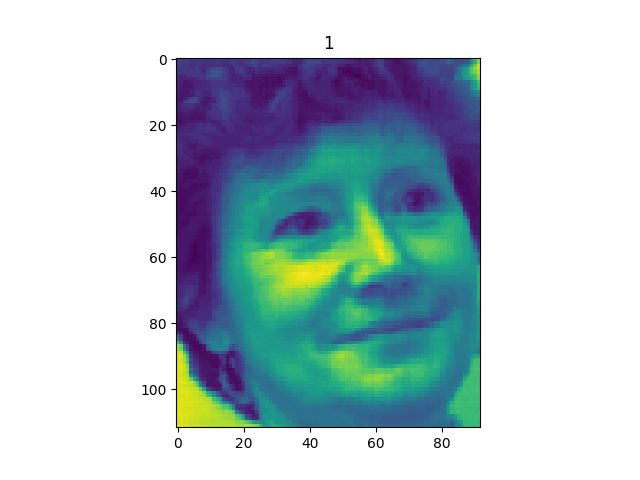
\includegraphics[width=.3\textwidth]{../project2/img/1.png}
%        \hspace{0.5in}
%        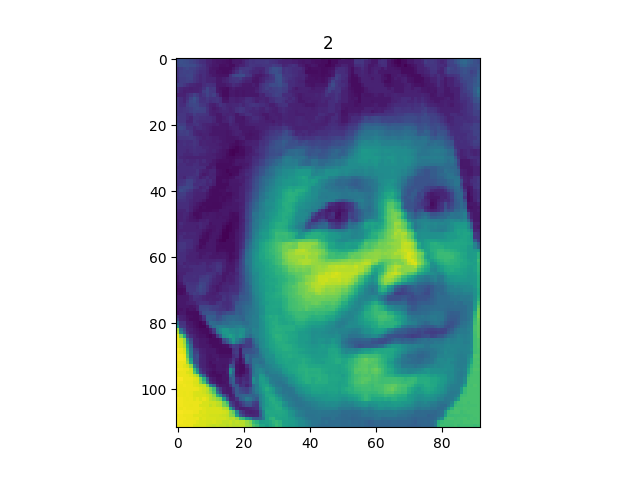
\includegraphics[width=.3\textwidth]{../project2/img/2.png}
%        \caption{Examples of 20-day Image with volume bar and moving average line}
%        \label{20-day image}
%    \end{figure}
%
%
%    Images labels take value \textbf{1} for positive returns and \textbf{0} for non-positive returns. In addition, we use \textbf{2} to mark the NaN value. In the simplest terms, you need to complete a two-class classification problem, and use the CNN model to predict whether the trend is 'down' or 'up' for the input image. For detail of data and label file, please refer to appendix.
%    
%    \item \textbf{Architecture Design}
%    
%    Why use CNN? Since CNN impose cross-parameter restrictions that dramatically reduce parameterization and embed a number of tools that make the model resilient to deformation and re-positioning of important objects in the image. A core building block consists of three operations: convolution, activation and pooling. In the paper, for 20-day image, they build a baseline CNN architectures with 3 conv blocks and connected with a fully connected layer as a classifier head. You should refer to the design of the conv block in the original paper (including the selection of the size of the convolution kernel, the selection of the convolution method, the design of the pooling layer and the selection of the activation function, etc) Figure \ref{cnn model} shows a diagram of 20-day CNN model proposed in the paper, just for your reference.
%    
%    \begin{figure}
%        \centering
%        \includegraphics[width=.25\textwidth, height=0.45\textwidth]{../project2/img/cnn.png}
%        \caption{Diagram of CNN model}
%        \label{cnn model}
%    \end{figure}
%    
%    \item \textbf{Working Flow}
%    
%    \begin{description}
%    \item[Data split] First, consider dividing the entire sample into training, validation and testing samples. In the original paper, they use first seven-year sample (1993-1999) to train and validate model, in which 70\% of the sample are randomly selected for training and the remaining 30\% for validation. The remaining twenty years of data  comprise the out-of-sample test dataset. You should consider follow the same format in case better comparson with the original paper.
%    
%    \item[Loss and evaluation] You can simply treat the prediction analysis as a classification problem. In particular, the label for an image is defined as y = 1 if the subsequent return is positive and y = 0 otherwise. The training step minimizes the cross-entropy loss, which is the standard objective function for classification problem, which define as:$$L_{CE}(y,\hat{y}) = -y\log(\hat{y}) - (1-y)log(1-\hat{y})$$ where $\hat{y}$ is the prediction and $y$ is the ground truth. 
%    
%    To measure the classification accuracy, a true positive (TP) (true negative (TN)) occurs when a predicted probability of greater than 50\% coincides with a positive realized return (a probability less than 50\% coincides with a negative return, respectively). False positives and negatives (FP and FN) are the complementary outcomes. We calculate classification accuracy as:$$Accuracy = (TP + TN)/(TP + TN + FP + FN)$$ For more evaluation metrics or methods, like Sharpe Ratio, please refer to the original paper.
%    
%    \item[Training process] The author adopt several ways to combat over-fitting issue and aid efficient computation. For example, they applied the Xavier initialization for weights in each layer, which guarantees faster convergence by scale the initial weights. Other techniques like dropout, batch normalization and early stopping may also improve performance. We recommend to refer to the training details mentioned in the paper 3.3 when training the baseline model.
%
%    \end{description}
%    
%    \item \textbf{Extensions}
%    
%    \begin{itemize}
%        \item For ablation studies and testing robustness, we suggest you follow what original paper mentioned in Appendix B. For example, you can perform the same sensitivity analysis of the CNN prediction model to alternate choices in model architecture (e.g. varying the number of filters in each layer or varying the number of layers, like the paper shows in Table 18) 
%        
%        \item Another direction that can be used as an extension is exploring of the interpretability of the CNN model in Chapter 6 of the original paper. Though interpreting a CNN model is quite difficult due to its stacks of non-linear structures, you can imitate what the author did in Part 6.3, using a visualization method (Grad-CAM) to understand how different image examples activate the regions of the CNN to trigger `up' or `down' return predictions.
%        
%        \item What's more, we encourage you not being limited to simple binary classification task, since the label files we provided consist more meaningful attributes, containing both categorical and numerical values. For example, you can use the same 20-day horizon images to train your model to predict the return trend of different subsequent \textbf{y}-days even the detailed return values. (\textbf{y} can be 5, 20 even larger). In this way, you can prove more firmly that using CNN can automatically identity robust and transferable predictive features.
%    \end{itemize}
%
%   
%\end{enumerate}
%
%
%\subsection{Empirical Asset Pricing via Machine Learning}
%
%The fundamental goal of asset pricing is to understand the behavior of risk premiums. However, risk premium is difficult to measure: market efficiency forces return variation to be dominated by unforecastable news that obscures risk premiums. This paper predicts the expected return and identifies informative predictor variables via machine learning methods, which facilitates more reliable investigation into economic mechanisms of asset pricing. Now you are required to replicate some results of this paper based your understanding of it, and write a report about your work.
%
%The requirements of this paper replication project are as follow:
%\begin{itemize}
%\item The machine learning methods used in this paper include linear regression (OLS, elastic net), dimension reduction (PLS, PCR), generalized linear models, trees (gradient boosting trees, random forest) and neural networks. Please try to replicate \textbf{at least 6 methods} of them (e.g., OLS, elastic net, PLS, PCR, random forest, neural networks, etc. Please note that if you choose OLS, OLS-3 should also be included; and if you choose neural network, NN1 to NN5 are included. Besides, robust loss function should also be considered. See details in the paper), and analyze your results specifically. Hints on parameter choice are presented in the paper.
%\item Include the variable importance (section 2.3 of the paper) in your analysis. You do not need to replicate all the figures in section 2.3, but you are encouraged to investigate it carefully.
%\item Note that this paper uses a `recursive performance evaluation scheme'. You are also required to evaluate your result by this method. For more details of this method, please refer to the paper and its supplementary material. The PPT presented in class about this project may also be helpful to you.
%\item As you can know from the paper (section 2.1), predictive characteristics include firm characteristics, sic code and macroeconomic predictors. Firm characteristics and sic code are provided in the original dataset of this paper, and the 8 macroeconomic predictors are constructed following Welch and Goyal (2008), which are not directly provided in the original dataset of this paper. Hence, you may construct the predictors by yourself according to the description in Welch and Goyal (2008), for instance, see \\
%\url{https://christophj.github.io/replicating/r/replicating-goyal-welch-2008/}.
%\item The portfolio forecast part of the paper (section 2.4) is not compulsory for you to replicate.
%\end{itemize}
%
%You may access the paper and the supplementary material via: \\
%\url{https://dachxiu.chicagobooth.edu/download/ML.pdf} \\
%or \\
%\url{https://academic.oup.com/rfs/article/33/5/2223/5758276}.  \\
%Meanings of characteristics of the data are provided in the supplementary material.
%
%The original dataset (4.05GB) can be obtained at \\ 
%\url{https://dachxiu.chicagobooth.edu/download/datashare.zip}. \\
%The zip file is about 1.64GB. Please be patient since it may take you about 6 hours to download the data. Another fast access can be via \\
%\url{https://www.dropbox.com/s/zzgjdubvv23xkfp/datashare.zip?dl=0}


%\section{Kaggle Contest: Home Credit Default Risk}
%
%Many people struggle to get loans due to insufficient or non-existent credit histories. And, unfortunately, this population is often taken advantage of by untrustworthy lenders.
%
%Home Credit strives to broaden financial inclusion for the unbanked population by providing a positive and safe borrowing experience. In order to make sure this underserved population has a positive loan experience, Home Credit makes use of a variety of alternative data--including telco and transactional information--to predict their clients' repayment abilities.
%
%While Home Credit is currently using various statistical and machine learning methods to make these predictions, they're challenging Kagglers to help them unlock the full potential of their data. Doing so will ensure that clients capable of repayment are not rejected and that loans are given with a principal, maturity, and repayment calendar that will empower their clients to be successful.
%
%Visit the following website to join the competition. 
%
%\url{https://www.kaggle.com/c/home-credit-default-risk/}

%{\bf Requirements}. For Kaggle contests, please register your team with name in the format of math6010z\_lastname, so that we could easily find your results on Kaggle. For example, a team with Shawn Zhu and Kate Wong would be named by math6010z\_Zhu\_Wong.



%Below are two candidate datasets. Challenge marked by * above is only optional. 
%
%\subsection{MNIST dataset -- a Warmup}
%
%Yann LeCun's website contains original MNIST dataset of 60,000 training images and 10,000 test images. 
%
%\url{http://yann.lecun.com/exdb/mnist/}
%
%There are various ways to download and parse MNIST files. For example, Python users may refer to the following website:
%
%\url{https://github.com/datapythonista/mnist}
%
%\noindent or MXNET tutorial on mnist
%
%\url{https://mxnet.incubator.apache.org/tutorials/python/mnist.html}
%
%\subsection{Fashion-MNIST dataset}
%
%Zalando's Fashion-MNIST dataset of 60,000 training images and 10,000 test images, of size 28-by-28 in grayscale. 
%
%\url{https://github.com/zalandoresearch/fashion-mnist}
%
%%As a reference, here is Jason Wu, Peng Xu, and Nayeon Lee's exploration on the dataset in project 1:
%
%%\url{https://deeplearning-math.github.io/slides/Project1_WuXuLee.pdf}
%
%
%\subsection{Identification of Raphael's paintings from the forgeries}
%
%The following data, provided by Prof. Yang WANG from HKUST,
%
%\url{https://drive.google.com/folderview?id=0B-yDtwSjhaSCZ2FqN3AxQ3NJNTA&usp=sharing}
%
%\noindent contains a 28 digital paintings of Raphael or forgeries. Note that there are both jpeg and tiff files, so be careful with the bit depth in digitization. The following file
%
%\url{https://docs.google.com/document/d/1tMaaSIrYwNFZZ2cEJdx1DfFscIfERd5Dp2U7K1ekjTI/edit}
%
%\noindent contains the labels of such paintings, which are 
%\begin{enumerate}
%\item[1] Maybe Raphael - Disputed
%\item[2] Raphael
%\item[3] Raphael
%\item[4] Raphael
%\item[5] Raphael
%\item[6] Raphael
%\item[7] Maybe Raphael - Disputed
%\item[8] Raphael
%\item[9] Raphael
%\item[10] Maybe Raphael - Disputed
%\item[11] Not Raphael
%\item[12] Not Raphael
%\item[13] Not Raphael
%\item[14] Not Raphael
%\item[15] Not Raphael
%\item[16] Not Raphael
%\item[17] Not Raphael
%\item[18] Not Raphael
%\item[19] Not Raphael
%\item[20] My Drawing (Raphael?)
%\item[21] Raphael
%\item[22] Raphael
%\item[23] Maybe Raphael - Disputed
%\item[24] Raphael
%\item[25] Maybe Raphael - Disputed
%\item[26] Maybe Raphael - Disputed
%\item[27] Raphael
%\item[28] Raphael
%\end{enumerate}
%There are some pictures whose names are ended with alphabet like A's, which are irrelevant for the project. 
%
%The challenge of Raphael dataset is: can you exploit the known Raphael vs. Not Raphael data to predict the identity of those 6 disputed paintings (maybe Raphael)? Textures in these drawings may disclose the behaviour movements of artist in his work. One preliminary study in this project can be: \emph{take all the known Raphael and Non-Raphael drawings and use leave-one-out test to predict the identity of the left out image; you may break the images into many small patches and use the known identity as its class.}      
%
%The following student poster report seems a good exploration
%
%\url{https://github.com/yuany-pku/2017_CSIC5011/blob/master/project3/05.GuHuangSun_poster.pdf}
%%\url{http://math.stanford.edu/~yuany/course/2015.fall/poster/Raphael_LI\%2CYue_1300010601.pdf}
%
%The following paper by Haixia Liu, Raymond Chan, and me studies Van Gogh's paintings which might be a reference for you:
%
%\url{http://dx.doi.org/10.1016/j.acha.2015.11.005}
%

%\newpage
%\section{Permutation Invariant and Equivariant Representations}
%$$
%\begin{array}{l}{\text { Definition 2.1. Let } G \text { be a group and } X \text { and } Y \text { two sets. We assume that } G \text { acts on } X \text { (resp. } Y) \text { by }} \\ {g \cdot x \text { (resp. } g * y) \text { for } g \in G \text { and } x \in X \text { (resp. } y \in Y) . \text { We say that a map } f : X \rightarrow Y \text { is }} \\ {\qquad \begin{array}{l}{\bullet G \text { -invariant if } f(g \cdot x)=f(x) \text { for any } g \in G \text { and any } x \in X} \\ {\bullet G \text { -equivariant if } f(g \cdot x)=g * f(x) \text { for any } g \in G \text { and any } x \in X}\end{array}}\end{array}
%$$
%
%Replace the translation convolution
%$$
%{\left[f * \psi^{i}\right](x)=\sum_{y \in \mathbb{Z}^{2}} \sum_{k=1}^{K^{l}} f_{k}(y) \psi_{k}^{i}(x-y)} $$
%by group-convolution [Cohen and Welling, https://arxiv.org/abs/1602.07576]
%$$
%{[f \star \psi](g)=\sum_{h \in G} \sum_{k} f_{k}(h) \psi_{k}\left(g^{-1} h\right)}
%$$
%
%When $G=S_{n}$ and the actions are induced by permutation, we call $G$-invariant (resp. G-equivariant) functions as permutation invariant (resp. permutation equivariant) functions. 
%
%{\bf Theorem 3.1}[Sannai, Takai, Cordonnier, https://arxiv.org/abs/1903.01939v2] (Kolmogorov-Arnold's representation theorem for permutation actions). Let $K \subset {\mathbb{R}^{n}}$ be a compact set. Then, any continuous $S_{n}$-invariant function $f : K \longmapsto \mathbb{R}$ can be represented as  
%$$ f\left(x_{1}, \ldots, x_{n}\right)=\rho\left(\sum_{i=1}^{n} \phi\left(x_{i}\right)\right), $$ 
%for some continuous function $\rho : \mathbb{R}^{n+1} \rightarrow \mathbb{R} $. Here, $\phi : \mathbb{R} \rightarrow \mathbb{R}^{n+1} ; x \mapsto\left(1, x, x^{2}, \ldots, x^{n}\right)^{\top}$. 
%
%$$
%\begin{array}{l}{\text { Proposition 4.1. A map } F : \mathbb{R}^{n} \rightarrow \mathbb{R}^{n} \text { is } S_{n} \text { is } S_{n} \text { and variant if and only if there is a Stab(1)-invariant }} \\ {\text { function } f : \mathbb{R}^{n} \rightarrow \mathbb{R} \text { satisfying } F=(f, f \circ(12), \ldots, f \circ(1 n))^{\top} \text { . Here, }(1 i) \in S_{n} \text { is the }} \\ {\text { transposition between 1 and i. }}\end{array}
%$$
%
%$$
%\begin{array}{l}{\text { Corollary } 4.1 \text { (Representation of Stab( } 1) \text { -invariant function). Let } K \subset \mathbb{R}^{n} \text { be } a \text { compact set, let }} \\ {f : K \longrightarrow \mathbb{R} \text { be a continuous and Stab }(1) \text { -invariant function. Then, } f(\boldsymbol{x}) \text { can be represented as }} \\ {\qquad f(\boldsymbol{x})=f\left(x_{1}, \ldots, x_{n}\right)=\rho\left(x_{1}, \sum_{i=2}^{n} \phi\left(x_{i}\right)\right)} \\ {\text { for some continuous function } \rho : \mathbb{R}^{n+1} \longrightarrow \mathbb{R} . \text { Here, } \phi : \mathbb{R} \rightarrow \mathbb{R}^{n} \text { is similar as in Theorem } 3.1}\end{array}
%$$

%\section{Air Quality Weibo Data} (courtesy of Prof. Xiaojin Zhu from University of Wisconsin at Madison) 
%You can login my server:
%
%\texttt{ssh einstein@162.105.205.92}
%
%\noindent using the password I provided on class. 
%
%On the read-only folder \texttt{/data/AQweibo/}, the \texttt{AQICityData/} directory contains the Weibo posts, the AQI for 108 cities with (AQI) information during the study period
%from 2013-11-18 to 2013-12-18 (both inclusive); Information for the spatiotempral bin (city,date) is in the directory \texttt{city\_date/}. See \texttt{README.txt} for more information.
%
%


%\section{Raph}
%The following data contains 1258-by-452 matrix with closed prices of 452 stocks in SNP'500 for workdays in 4 years.
%
%\url{http://math.stanford.edu/~yuany/course/data/snp452-data.mat} 
%
%\noindent or in R: 
%
%\url{http://math.stanford.edu/~yuany/course/data/snp500.Rda}
%
%%You may use PCA to explore the `invisible hands' of markets.
%
%\section{Animal Sleeping Data} The following data contains animal sleeping hours together with other features: 
%
%\url{http://math.stanford.edu/~yuany/course/data/sleep1.csv}
%
%
%\section{US Crime Data} The following data contains crime rates in 59 US cities during 1970-1992:
%
%\url{http://math.stanford.edu/~yuany/course/data/crime.zip}
%
%\noindent Some students in previous classes study crime prediction in comparison with MLE and James-Stein, for example, see
%
%\url{https://github.com/yuany-pku/2017_math6380/blob/master/project1/DongLoXia_slides.pptx}
%
%
%\section{NIPS paper datasets}
%NIPS is one of the major machine learning conferences. The following datasets collect NIPS papers:
%
%\subsection{NIPS papers (1987-2016)} The following website: 
%
%\url{https://www.kaggle.com/benhamner/nips-papers}
%
%\noindent collects titles, authors, abstracts, and extracted text for all NIPS papers during 1987-2016. In particular the file {\texttt{paper\_authors.csv}} contains a sparse matrix of paper coauthors. 
%
%\subsection{NIPS words (1987-2015)} The following website:
%
%\url{https://archive.ics.uci.edu/ml/datasets/NIPS+Conference+Papers+1987-2015}
%
%\noindent collects the distribution of words in the full text of the NIPS conference papers published from 1987 to 2015. The dataset is in the form of a 11463 x 5812 matrix of word counts, containing 11463 words and 5811 NIPS conference papers (the first column contains the list of words). Each column contains the number of times each word appears in the corresponding document. The names of the columns give information about each document and its timestamp in the following format: {\texttt{Xyear\_paperID}}. 
%
%
%\section{Jiashun Jin's data on Coauthorship and Citation Networks for Statisticians}
%Thanks to Prof. Jiashun Jin at CMU, who provides his collection of citation and coauthor data for statisticians. The data set covers all papers between 2003 and the first quarter of 2012 from the Annals of Statistics, Journal of the American Statistical Association, Biometrika and Journal of the Royal Statistical Society Series B. The paper corrections and errata are not included. There are 3607 authors and 3248 papers in total. The zipped data file (14M) can be found at 
%
%\url{http://math.stanford.edu/~yuany/course/data/jiashun/Jiashun.zip}
%
%\noindent with an explanation file
%
%\url{http://math.stanford.edu/~yuany/course/data/jiashun/ReadMe.txt}
%
%With the aid of Mr. LI, Xiao, a subset consisting 35 COPSS award winners (\url{https://en.wikipedia.org/wiki/COPSS_Presidents\%27_Award}) up to 2015, is contained in the following file
%
%\url{http://math.stanford.edu/~yuany/course/data/copss.txt} 
%
%\noindent An example was given in the following article, A Tutorial of Libra: R Package of Linearized Bregman Algorithms in High Dimensional Statistics, downloaded at
%
%\url{http://math.stanford.edu/~yuany/course/reference/Libra_Tutorial_springer.pdf}
%
%The citation of this dataset is: \emph{P. Ji and J. Jin. Coauthorship and citation networks for statisticians. Ann. Appl. Stat. Volume 10, Number 4 (2016), 1779-1812}, (\url{http://projecteuclid.org/current/euclid.aoas})
%
%
%
%
%\section{Co-appearance data in novels: Dream of Red Mansion and Journey to the West}
%
%A 374-by-475 binary matrix of character-event can be found at the course website, in .XLS, .CSV, .RData, and .MAT formats. For example the RData format is found at
%
%\url{http://math.stanford.edu/~yuany/course/data/dream.RData} 
%
%\noindent with a readme file:
%
%\url{http://math.stanford.edu/~yuany/course/data/dream.Rd}
%
%\noindent as well as the .txt file which is readable by R command {\tt read.table()},
%
%\url{http://math.stanford.edu/~yuany/course/data/HongLouMeng374.txt}
%
%\url{http://math.stanford.edu/~yuany/course/data/readme.m}
%
%Thanks to Ms. WAN, Mengting, who helps clean the data and kindly shares her BS thesis for your reference
% 
%\url{http://math.stanford.edu/~yuany/report/WANMengTing2013_HLM.pdf}
%
%%Among various choices of analysis, with this data matrix $X$, you may form a weighted graph $W=X * X'$, pursue PCA of $X$, and sparse SVD of $X$ etc. As an example, here is a project presentation by LI, Liying which gives an analysis of A Journey to the West (by Chen-En Wu) based on PCA, for the class Mathematical Introduction to Data Science in Fall 2012 where you may find more interesting approaches.
%%
%%\url{http://www.math.pku.edu.cn/teachers/yaoy/reference/LiyingLI_Xiyouji2012_slides.pdf}
%
%Moreover you may find a similar matrix of 302-by-408 for the Journey to the West (by Chen-En Wu) at:
%
%\url{http://math.stanford.edu/~yuany/course/data/west.RData}
%
%\noindent whose matlab format is saved at
%
%\url{http://math.stanford.edu/~yuany/course/data/xiyouji.mat}

%%%%%%


%\section{Drug Efficacy Data}
%
%Thanks to Prof. Xianting Ding at Shanghai Jiao Tong University and Prof. Chih-Ming Ho from University of California at Los Angeles, we have the following datasets on combinatorial drug efficacy.
%
%The first dataset consists of two experiments, all with the same 4 drugs in cell lines for attacking leukemia, with 256 experiments of combinatorial drug dosage at 4 levels. The response is the therapeutic window measuring the efficacy with a trade-off by toxicity. 
% 
% \url{http://math.stanford.edu/~yuany/course/data/Ding_4drugs.xlsx}
%
%\noindent whose drugs are explained in 
%
%\url{http://math.stanford.edu/~yuany/course/data/Ding_4drugs_readme.pdf}
%
%Can you find a good prediction of drug response efficacy using those combinatorial dosage levels? It was suggested that quadratic polynomials at logarithmic dosage levels are good models in personalized medicine, e.g. the following cover paper in Science \emph{Translation Medicine}:
%
%\url{http://stm.sciencemag.org/content/8/333/333ra49}
%
%\noindent with a sample 14 drug efficacy at level 2 experiment data in liver transplant: 
%
%\url{http://math.stanford.edu/yuany/course/data/TB-FSC-03A-data.xlsx}

%\section{Drug Sensitivity Data by Cleave}
%The following dataset is kindly provided by Cleave Co. Ltd. USA, for the exploration on class. {\textbf{Please keep its use only in this class and any publication will be subject to the approval of Cleave.}}
%
%The dataset is contained in the following zip file (73M).
%
%\url{http://math.stanford.edu/~yuany/course/data/cleave.zip}
%
%\noindent where you may find
%\begin{enumerate}
%\item \texttt{data explanation.pptx}: description of data in pptx
%\item \texttt{data for Yuan Yao.xlsx}: data file
%\item \texttt{Gene set collection 1 for Yuan Yao.txt}: gene set collection
%\item \texttt{Gene set collection 2 for Yuan Yao.txt}: gene set collection
%\item \texttt{reference}: a folder contains a survey paper on 40+ machine learning algorithms as well as some source codes -- \emph{Nature Biotechnology 32, 1202--1212 (2014)} (\url{http://www.nature.com/nbt/journal/v32/n12/full/nbt.2877.html})
%\end{enumerate}
%
%The basic problem is to predict the drug response \texttt{IC50 within 72 hours}, using all the information collected so far, introduced by Ms. Lijing Wang with slides
%
%\url{http://math.stanford.edu/~yuany/course/2016.spring/cleave_lijing.pdf}
%
%\noindent as well as our CPH'2017 poster
%
%\url{http://math.stanford.edu/~yuany/publications/poster_CleaveBioCPH2017_ForReview.pdf}
%
%\noindent where the crucial discovery is that recursive variable selection by LASSO is more effective than one-stage LASSO. 

%\subsection{The Characters in A Dream of Red Mansion} 
%
%A 376-by-475 matrix of character-event can be found at the course website, in .XLS, .CSV, and .MAT formats. For example the Matlab format is found at
%
%\url{http://www.math.pku.edu.cn/teachers/yaoy/data/hongloumeng/hongloumeng376.mat} 
%
%\noindent with a readme file:
%
%\url{http://www.math.pku.edu.cn/teachers/yaoy/data/hongloumeng/readme.m}
%
%Thanks to Ms. WAN, Mengting (now at UIUC), an update of data matrix consisting 374 characters (two of 376 are repeated) which is readable by R read.table() can be found at 
%
%\url{http://www.math.pku.edu.cn/teachers/yaoy/data/hongloumeng/HongLouMeng374.txt}
%
%\noindent She also kindly shares her BS thesis for your reference
% 
% \url{http://www.math.pku.edu.cn/teachers/yaoy/reference/WANMengTing2013_HLM.pdf}
%
%% Among various choices of analysis, with this data matrix $X$, you may form a weighted graph $W=X * X'$, pursue PCA of $X$. 
%
%\subsection{A Journal to the West} On course website, you may also find the link to this dataset with a 302-by-408 matrix, whose matlab format is saved at
%
%\url{http://www.math.pku.edu.cn/teachers/yaoy/Fall2011/xiyouji/xiyouji.mat}
%
%For your reference, here is a project presentation by Mr. LI, Liying (at PKU) which gives an analysis based on PCA
%
%\url{http://www.math.pku.edu.cn/teachers/yaoy/reference/LiyingLI_Xiyouji2012_slides.pdf}
%

%\section{Heart PCI Operation Effect Prediction}
%
%The following data, provided by Dr. Jinwen Wang at Anzhen Hospital, 
%
%\url{http://math.stanford.edu/~yuany/course/data/heartData_20140401.xlsx}
%
%\noindent contains 2581 patients with 73 measurements (inputs) as well as a response variable indicating if after the heart operation there is a null-reflux state. This is a classification problem, with a challenge from the large amount of missing values. Sheet 3 and 4 in the file contains some explanation of the data and variables. 
%
%The problems are listed here:
%\begin{enumerate}
%\item The inputs (covariates) are of three kinds, measurements upon check-in, measurements before PCI operation, and measurements in PCI operations. For doctors, it is desired to find a prediction model based on measurements before the operation (including check-in). Sheet 2 in the file contains only such measurements.
%\subitem The following two reports by LV, Yuan and LI, Xiao, respectively, might be interesting to you:
%
%\url{http://math.stanford.edu/~yuany/course/reference/MSThesis.LvYuan.pdf} 
%
%\url{http://arxiv.org/abs/1511.04656} 
%
%\item It is also an interesting problem how to predict the effect based on all measurements, with lots of missing values. Sheet 1 contains the full measurements. There are some good work by previous students, which are listed here for your reference: 
%%\subitem The following two reports by LU, Yu and WANG, Qing, are probably inspiring to you.
%%
%%\url{http://www.math.pku.edu.cn/teachers/yaoy/reference/LuYu_201303_BigHeart.pdf} 
%%
%%\url{http://www.math.pku.edu.cn/teachers/yaoy/reference/WangQing_201303_BigHeart.pdf} 
%
%\subitem The following report by MIAO, Wang and LI, Yanfang, pioneers in missing value treatment. 
%
%\url{http://math.stanford.edu/~yuany/course/reference/MiaoLi2013S_project01.pdf}
%
%\end{enumerate} 

%\emph{In the final project, it is desired to take only those measurements upon check-in to predict the probability of non-reflux (non-reflow) after PCI operations. An interpretable model adds a big value! You may compare with your first warm-up project to show your improvements.} 
%
%
%\section{SNPs Data}
% This dataset contains a data matrix $X\in \R^{p\times n}$ of about $n=650,000$ columns of SNPs (Single Nucleid Polymorphisms) and $p=1064$ rows of peoples around the world. Each element is of three choices, $0$ (for `AA'), $1$ (for `AC'), $2$ (for `CC'), and some missing values marked by $9$. 
%
%\url{http://math.stanford.edu/~yuany/course/ceph_hgdp_minor_code_XNA.txt.zip}
%
%\noindent which is big (151MB in zip and 2GB original txt). Moreover, the following file contains the region where each people comes from, as well as two variables {\texttt{ind1}} and{\texttt{ind2}} such that $X({\texttt{ind1}},{\texttt{ind2}})$ removes all missing values. 
%
%\url{http://math.stanford.edu/~yuany/course/data/HGDP_region.mat}
%
%\noindent More detailed information about these persons in the dataset can be also found at
%
%\url{http://math.stanford.edu/~yuany/course/data/HGDPid_populations_ALL.xls}
%
%Some results by PCA can be found in the following paper, Supplementary Information. 
%
%\url{http://www.sciencemag.org/content/319/5866/1100.abstract}
%
%\section{Protein Folding} 
%Consider the 3D structure reconstruction based on incomplete MDS with uncertainty. Data file: 
%
%\url{http://math.stanford.edu/~yuany/course/data/protein3D.zip}
%
%\begin{figure}[htbp]
%\begin{center}
%\includegraphics[width=0.5\textwidth]{../2013_Spring_PKU/Yes_Human.png}  
%\caption{3D graphs of file PF00018\_2HDA.pdf (YES\_HUMAN/97-144, PDB 2HDA)}
%\label{yes_human}
%\end{center}
%\end{figure}
%
%\noindent In the file, you will find 3D coordinates for the following three protein families: 
%\subitem PF00013 (PCBP1\_HUMAN/281-343, PDB 1WVN), \\
%\subitem PF00018 (YES\_HUMAN/97-144, PDB 2HDA), and \\
%\subitem PF00254 (O45418\_CAEEL/24-118, PDB 1R9H). \\
%
%For example, the file {\tt PF00018\_2HDA.pdb} contains the 3D coordinates of alpha-carbons for a particular amino acid sequence in the family, YES\_HUMAN/97-144, read as
%
%{\tt{VALYDYEARTTEDLSFKKGERFQIINNTEGDWWEARSIATGKNGYIPS}}
%
%\noindent where the first line in the file is 
%
%97	V	0.967	18.470	4.342
%
%\noindent Here
%\begin{itemize}
%\item `97': start position 97 in the sequence
%\item `V': first character in the sequence
%\item $[x,y,z]$: 3D coordinates in unit $\AA$.
%\end{itemize}
%
%\noindent Figure \ref{yes_human} gives a 3D representation of its structure. 
%
%
%Given the 3D coordinates of the amino acids in the sequence, one can computer pairwise distance between amino acids, $[d_{ij}]^{l\times l}$ where $l$ is the sequence length. A \emph{contact map} is defined to be a graph $G_\theta=(V,E)$ consisting $l$ vertices for amino acids such that and edge $(i,j)\in E$ if $d_{ij} \leq \theta$, where the threshold is typically $\theta=5\AA$ or $8\AA$ here. 
%
%Can you recover the 3D structure of such proteins, up to an Euclidean transformation (rotation and translation), given noisy pairwise distances restricted on the contact map graph $G_\theta$, i.e. given noisy pairwise distances between vertex pairs whose true distances are no more than $\theta$? Design a noise model (e.g. Gaussian or uniformly bounded) for your experiments. 
%
%When $\theta=\infty$ without noise, classical MDS will work; but for a finite $\theta$ with noisy measurements, SDP approach can be useful. You may try the matlab package SNLSDP by Kim-Chuan Toh, Pratik Biswas, and Yinyu Ye, downladable at \url{http://www.math.nus.edu.sg/~mattohkc/SNLSDP.html}. 
%


%Attention: this last dataset is relatively big with about 2GB size. 
%
%You can login my server:
%
%\texttt{ssh einstein@162.105.205.92}
%
%\noindent using the password I provided on class. On the read only folder \texttt{/data/snp/}, you will find all the data in both .txt and .mat (\texttt{data.mat, HGDP\_region.mat, readme.m}).



%\subsection{Bird Flu Dataset} (courtesy of Steve Smale and Cissy) This dataset 162 H5N1 (bird flu) virus sequences discovered around the world:
%
%\url{http://www.math.pku.edu.cn/teachers/yaoy/data/birdflu_seq162.txt} 
%
%Locations of such virus discovered are reported with latitude and longitude coordinates on the globe:
%
%\url{http://www.math.pku.edu.cn/teachers/yaoy/data/birdflu_latgrat.txt} 
%
%Pairwise geodesic distances between these 162 sites are constructed as  
%
%\url{http://www.math.pku.edu.cn/teachers/yaoy/data/birdflu_geodist.txt}
%
%A kernel-induced $l_2$-distances between 162 virus sequences are given in 
%
%\url{http://www.math.pku.edu.cn/teachers/yaoy/data/birdflu_l2dist.txt}

\newpage

\section*{Peer Review}

In this exercise of open peer review, please write down your comments of the \emph{reports rather than of your own team} in the following format. Be considerate and careful with a precise description, avoiding offensive language. 

{\bf Deadline is \emph{11:59pm Saturday April 9, 2022}}. Submit your review in plain text to {\bf Canvas}. Rebuttal is open afterwards. %the email address (\url{aifin.hkust@gmail.com}) with title: \underline{MSBD5013: Project 1 Review}. Rebuttal is open afterwards.


%Your review assignment can be found at

%{\centering{\url{https://deeplearning-math.github.io/2019/project1/project1review_assignment.pdf} }}

%\noindent where each student (SID) is randomly assigned with 5 group reports (excluding your own reports). You should submit reviews at least for these assignments, but more reviews are welcome with additional bonus credit. 

%You should put each review in a plain text separately with a title  comprising the corresponding group number (\textbf{not your own group}) and your name (e.g., \emph{\underline{rev1\_group03\_Ian\_Goodfellow.pdf}}). Submit all your reviews in a single zip file \textbf{using canvas}. Rebuttal is open afterwards.

\begin{itemize}
\item Summary of the report.
\item Describe the strengths of the report. 
\item Describe the weaknesses of the report.
\item Evaluation on Clarity and quality of writing (1-5): Is the report clearly written? Is there a good use of examples and figures? Is it well organized? Are there problems with style and grammar? Are there issues with typos, formatting, references, etc.? Please make suggestions to improve the clarity of the paper, and provide details of typos.
\item Evaluation on Technical Quality (1-5): Are the results technically sound? Are there obvious flaws in the reasoning? Are claims well-supported by theoretical analysis or experimental results? Are the experiments well thought out and convincing? Will it be possible for other researchers to replicate these results? Is the evaluation appropriate? Did the authors clearly assess both the strengths and weaknesses of their approach? Are relevant papers cited, discussed, and compared to the presented work?
\item Overall rating: (5- My vote as the best-report. 4- A good report. 3- An average one. 2- below average. 1- a poorly written one). 
\item Confidence on your assessment (1-3)
(3- I have carefully read the paper and checked the results, 2- I just browse the paper without checking the details, 1- My assessment can be wrong)
\end{itemize}

%%
%%%Then please vote your top THREE favourite reports on Doodle: 
%%%\url{xxx}
%%
\newpage

\section*{Rebuttal}
The rebuttal period starts from now, till \emph{11:59pm Saturday April 16, 2022}. Restrict the number of characters of your rebuttal within {\bf{5,000}}. Submit your rebuttal in PLAIN TEXT or PDF format to \textbf{canvas} with filename comprising the corresponding group number: e.g. \underline{rebuttal1\_group02.pdf}. %(\href{mailto:datascience.hw@gmail.com}{datascience.hw@gmail.com}) with Title: \underline{CSIC 5011: Project 1 Rebuttal}.

The following tips of rebuttal might be helpful for you to follow:

1. The main aim of the rebuttal is to answer any specific questions that the reviewers might have raised, or to clarify any misunderstanding of the technical content of the paper.

2. Keep your rebuttal short, to-the-point, and specific. In our experience, such rebuttals have the maximum impact.

3. Always be polite and professional. Refrain from name calling or rude comments, especially in response to negative reviews.

4. Highlight the changes in your manuscripts had you made a simple revision.

%

\end{document}


